\section{Definition of Return}
In everyday language, the \emph{return} of an asset refers to how much money one gains or loses by holding that asset over some specific period. Let us formalize this concept.

\subsection{Return}
Suppose you buy an asset (e.g., a stock) at price $P_0$ at the beginning of the period, and at the end of the period the price is $P_1$. If the asset pays some dividend $D$ during that period (for instance, a stock dividend), then the total \emph{payout} is $P_1 + D$. The \textbf{discrete return} $R$ is defined by
$$
R = \frac{P_1 + D - P_0}{P_0}.
$$
In other words, it is the fractional (or percentage) change in value (price plus any distributed income) over the initial price. If $R$ is positive, the asset gained value; if $R$ is negative, it lost value.

For example, if $P_0 = 100\,$\$ (the asset costs 100 dollars initially) and at the end of the period $P_1 = 103\,$\$, with a $1\,$\$ dividend paid, then
$$
R = \frac{103 + 1 - 100}{100} = \frac{4}{100} = 0.04,
$$
meaning a $4\%$ return over that period.

\subsection{Randomness of Returns}
Asset prices fluctuate due to various uncertainties (market conditions, news events, etc.), so returns are treated as \emph{random variables}. For each asset $i$, we usually denote its \emph{return} in a particular period by $R_t^{(i)}$. The exact realization of $R_t^{(i)}$ is not known in advance, but we can estimate or model its distribution based on historical data, economic models, or other forecasting methods.


\section{Definition of a Portfolio}
In finance, an \textbf{asset} is anything that can generate a (random) return over time, such as a stock, a bond, or any financial instrument. Suppose we have $n$ assets, each with a random return denoted by $R^{(i)}$ for $i = 1, 2, \ldots, n$. Then, in the universe of assets, the random vector of returns is:
$$
\mbf R = (R^{(1)}, R^{(2)}, \ldots, R^{(n)})
$$
A \textbf{portfolio} is a collection of positions (or allocations) in these $n$ assets. Mathematically, a portfolio can be represented by a vector of \textbf{weights}:
$$
\mbf w = (w_1, w_2, \ldots, w_n),
$$
where $w_i$ is the fraction of total capital invested in asset $i$. Typically, we impose the constraint
$$
\mbf w\'\mbf 1=\sum_{i=1}^n w_i = 1,
$$
meaning that 100\% of the available capital is allocated across these assets (no leftover money). In many settings, we also require $w_i \ge 0$ to forbid short-selling (i.e., holding negative positions in any asset).
The returns of the portfolio are given by: 
$$
R^p := \mbf w\' \mbf R = \sum_{i=1}^n w_i R^{(i)}
$$

\section{Expected Returns and Covariance of Returns}
Let $R^{(i)}$ be the random return of asset $i$. By \emph{return} we mean the percentage gain (or loss) over some reference period (e.g., one day, one month, one year). In finance, we usually treat each $R^{(i)}$ as a random variable with a certain probability distribution. 

\subsection{Expected Return Vector}
We define $\b \mu := \E[\mbf R] $ as the vector of \textbf{expected returns}. That is, 
$$\begin{array}{cc}
\b \mu 
=
\1{\v{\mu_1 \\ \mu_2 \\ \ldots \\  \mu_n}}
:=
\1{
\v{
\E[R^{(1)}] \\ \E[R^{(2)}] \\ \vdots \\ \E[R^{(n)}]
}
}
\end{array}$$
where
$
\mu_i = \mathbb{E}[R^{(i)}]
$ is the expected return of asset $i$. 
Given a portfolio with weights $\mbf w$, the \textbf{expected return of the portfolio} is
$$
\E[R^p] =
\E[\mbf w\'\mbf R] 
=
\mbf w^\top \E[\mbf R] = \mbf w\' \b \mu 
$$

\subsection{Covariance Matrix}
The \textbf{risk} in returns is usually represented by the \textbf{variance} and \textbf{covariance} of the random variables $R^{(i)}$. We define the \textbf{covariance matrix} $\mbf  \Sigma$ of the returns $R^{(1)}, R^{(2)}, \ldots, R^{(n)}$ as the $n \times n$ matrix whose entries are
$$
\Sigma_{ij} = \mathrm{Cov}(R^{(i)}, R^{(j)}).
$$
That is,
$$
\mbf  \Sigma := \begin{pmatrix}
\mathrm{Var}(R^{(1)}) & \mathrm{Cov}(R^{(1)}, R^{(2)}) & \cdots & \mathrm{Cov}(R^{(1)}, R^{(n)}) \\
\mathrm{Cov}(R^{(2)}, R^{(1)}) & \mathrm{Var}(R^{(2)}) & \cdots & \mathrm{Cov}(R^{(2)}, R^{(n)}) \\
\vdots & \vdots & \ddots & \vdots \\
\mathrm{Cov}(R^{(n)}, R^{(1)}) & \mathrm{Cov}(R^{(n)}, R^{(2)}) & \cdots & \mathrm{Var}(R^{(n)})
\end{pmatrix}.
$$
The \textbf{variance of the portfolio} with weights $\mbf w$ is then given by
$$
\mathrm{Var}[R^p]=
\mathrm{Var}[\mbf w\' \mbf R]=
\mbf w\'\mathrm{Var}[\mbf R] \mbf w\
= \mbf w\' \mbf \Sigma \, \mbf w.
$$

\subsection{Mean--Variance Representation of Assets}
In economics and finance, it is very common to characterize assets by two key moments of their return distributions: the \emph{mean} (expected return) and the \emph{standard deviation} (volatility). This approach underpins the so-called \emph{mean--variance} framework originally proposed by Harry Markowitz. 

\subsubsection{Plotting Assets in the Mean--Standard Deviation Plane}
Let $R^{(i)}$ denote the random return of asset $i$, and let
\[
\mu_i \;=\;\E[R^{(i)}]
\quad\text{and}\quad
\sigma_i \;=\;\sqrt{\mathrm{Var}[R^{(i)}]}.
\]
In the simplest case, one represents each asset by a single point in the $(\sigma,\,\mu)$ plane:
\[
(\,\sigma_i,\,\mu_i\,).
\]
Geometrically:
\begin{itemize}
    \item \(\sigma_i\) (on the $x$-axis) measures the volatility or total risk of the asset.
    \item \(\mu_i\) (on the $y$-axis) measures the expected return (or average profit/loss) of the asset.
\end{itemize}
Hence, each asset can be visualized as a point in this mean--standard deviation space. 

\subsubsection{From Single Assets to Portfolios}
A \emph{portfolio} of multiple assets also has an expected return and a standard deviation. Specifically, if $\mbf w$ is the vector of portfolio weights and $\mbf R=(R^{(1)},\dots,R^{(n)})$ is the random vector of returns on the $n$ assets, then:
\[
\text{Mean of the portfolio} \;=\; 
\E[R^p] 
~\equiv~ 
\mbf w^\top\,\b\mu,
\qquad
\text{Std.\ dev.\ of the portfolio} \;=\;
\sqrt{\mbf w^\top\,\mbf \Sigma\,\mbf w}.
\]
Thus, any feasible portfolio \(\mbf w\) is mapped to a point \(\bigl(\sqrt{\mbf w^\top\,\mbf \Sigma\,\mbf w},\;\mbf w^\top \b\mu\bigr)\) in the same mean--standard deviation plane. The \emph{efficient frontier} is precisely the set of portfolios that achieve the highest \(\mbf w^\top \b\mu\) for a given level of \(\sqrt{\mbf w^\top \mbf \Sigma \mbf w}\), or equivalently, the smallest \(\sqrt{\mbf w^\top \mbf \Sigma \mbf w}\) for a given \(\mbf w^\top \b\mu\).


\begin{figure}[H]
  \centering
  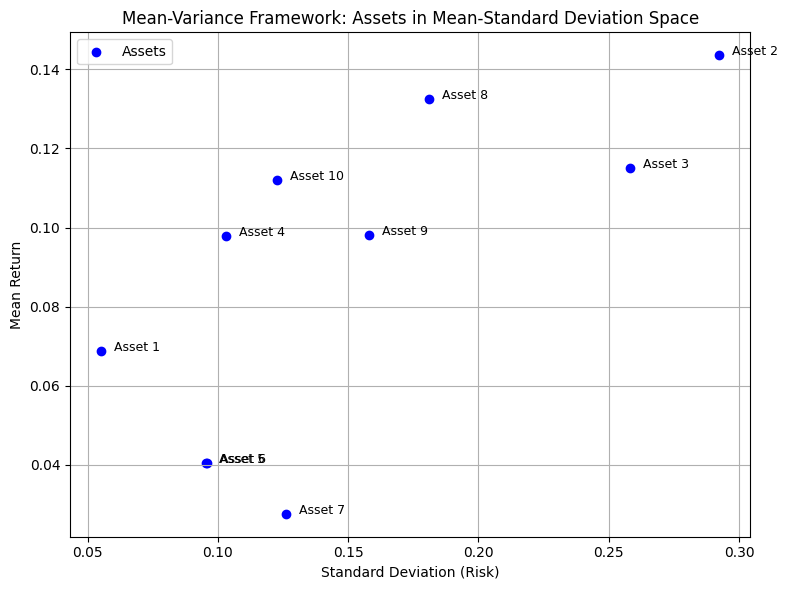
\includegraphics[scale=0.7]{points.png}
%  \caption{}
\end{figure}


\section{The Markowitz Problem}
In his seminal work, Harry Markowitz proposed balancing expected return against variance of returns to obtain an \emph{efficient portfolio}. The classical \textbf{Markowitz mean--variance optimization problem} can be expressed in multiple equivalent ways; one common formulation is:

\subsection{Minimize Variance Subject to a Target Return}

$$
\mbf w(\red{\mu_{\arg \min}}):=
\2{\begin{array}{rl}
\underset{\mbf w}{\arg \min} & \V [R^p]
\\ [1em]
\t{s.t.} & 
	\left|
	\begin{array}{rl}
	\E[R^p] &\geq \red{\mu_{min}}
	\\
	\sum_{i=1}^n w_i &= 1
	\\
	\brown{w_i} & \brown{\geq 0 ~~\forall i}
	\end{array}
	\right.
\end{array}
}
=
\2{\begin{array}{rl}
\underset{\mbf w}{\arg \min} & \mbf w\'\mbf \Sigma \mbf w
\\ [1em]
\t{s.t.} & 
	\left|
	\begin{array}{rl}
	\mbf w\'\b \mu  &\geq \red{\mu_{min}}
	\\
	\mbf w\'\mbf 1 &= 1
	\\
	\brown{\mbf w} & \brown{\geq \mbf 0}
	\end{array}
	\right.
\end{array}
}
$$
where:
\begin{itemize}
    \item $\mbf w = (w_1, \ldots, w_n)$ are the portfolio weights,
    \item $\mbf \Sigma$ is the covariance matrix of returns,
    \item $\b \mu$ is the vector of expected returns,
    \item $\red{\mu_{min}}$ is the minimum acceptable (target) return for the portfolio,
    \item $\mbf w\'\mbf 1 =\sum_{i=1}^n w_i = 1$ enforces that all our capital (100\%) is fully invested
    \item \brown{Optionally, $w_i \ge 0$ disallows short-selling.}
\end{itemize}
The solution to $\mbf w(\red{\mu_{\min}})$ yields the portfolio with the minimal variance among all that satisfy the target return $\red{\mu_{\min}}$. As we solve $\mbf w(\red{\mu_{\min}})$ for different values of $\red{\mu_{\min}}$, we sweep out the efficient frontier.


\begin{figure}[h!]
  \centering
  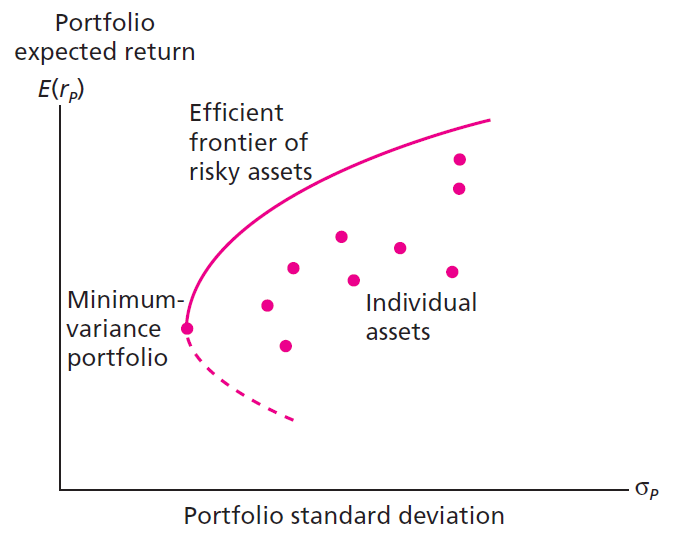
\includegraphics[scale=0.5]{efficient_frontier.png}
%  \caption{}
\end{figure}



\subsection{Alternative Formulations}
Other commonly used approaches revolve around the same concept of trading off risk and reward:
\begin{itemize}
    \item \textbf{Maximize expected return subject to a maximum risk:}

$$
\mbf w(\red{\sigma^2_{max}})
:=
\2{\begin{array}{rl}
\underset{\mbf w}{\arg \max} & \E [R^p]
\\[1em]
\t{s.t.} & 
	\left|
	\begin{array}{rl}
	\V[R^p] &\leq \red{\sigma_{\max}^2}
	\\
	\sum_{i=1}^n w_i &= 1
	\\
	\brown{w_i} &\brown{\geq 0 ~~\forall i}
	\end{array}
	\right.
\end{array}
}
=
\2{\begin{array}{rl}
\underset{\mbf w}{\arg \max} & \mbf w\'\b \mu 
\\ [1em]
\t{s.t.} & 
	\left|
	\begin{array}{rl}
	\mbf w\'\mbf \Sigma \mbf w &\leq \red{\sigma_{\max}^2}
	\\
	\mbf w\'\mbf 1 &= 1
	\\
	\brown{\mbf w} & \brown{\geq \mbf 0}
	\end{array}
	\right.
\end{array}
}
$$
where $\red{\sigma^2_{max}}$ is the maximum acceptable variance for the portfolio. As we solve $\mbf w(\red{\sigma^2_{max}})$ for diffent values of $\red{\sigma^2_{max}}$ we sweep out the efficient frontier.
    
    \item \textbf{Mean--variance parametrization:} 
$$
\mbf w(\red{\lambda}):=
\2{\begin{array}{rl}
\underset{\mbf w}{\arg \min} & \V[R^p] - \red{\lambda} \E [R^p]
\\ [1em]
\t{s.t.} & 
	\left|
	\begin{array}{rl}
	\sum_{i=1}^n w_i &= 1
	\\
	\brown{w_i} &\brown{\geq 0 ~~\forall i}
	\end{array}
	\right.
\end{array}
}
=
\2{\begin{array}{rl}
\underset{\mbf w}{\arg \min} & 
\mbf w\'\mbf \Sigma \mbf w - \red{\lambda} \mbf w\'\b \mu 
\\ [1em]
\t{s.t.} & 
	\left|
	\begin{array}{rl}
	\mbf w\'\mbf 1 &= 1
	\\
	\brown{\mbf w} & \brown{\geq \mbf 0}
	\end{array}
	\right.
\end{array}
}
$$
where $\red \lambda > 0$ is a parameter that encodes the investor's risk aversion. By solving $\mbf w(\red \lambda)$ for different values of $\red \lambda$, we sweep out the efficient frontier.
\end{itemize}

These formulations are all \emph{equivalent} in the sense that they generate the same \emph{efficient frontier} in the plane of $(\text{variance}, \text{expected return})$. The choice of formulation depends on how one prefers to express constraints (fixing a minimum return vs.\ a maximum risk vs.\ a parametric trade-off).


\section{Empirical Implementation} 
In practice, implementing the Markowitz model requires obtaining historical asset returns data, estimating expected returns and the covariance matrix, and then solving the corresponding optimization problem numerically. 

\subsection{Data and Parameter Estimation}
\begin{enumerate}
    \item \textbf{Historical Prices:} Collect daily (or monthly, quarterly, etc.) asset prices for each of the $n$ assets over a chosen lookback window (e.g., the past 20 years).
    \item \textbf{Compute Returns:} For each asset $i$ at each time step $t$, compute the discrete return
    $$
        R_t^{(i)} = \frac{P_t^{(i)} + D_t^{(i)} - P_{t-1}^{(i)}}{P_{t-1}^{(i)}},
    $$
    where $P_t^{(i)}$ is the price of asset $i$ at time $t$ and $D_t^{(i)}$ is any dividend (if relevant).
    \item \textbf{Expected Returns:} For each period $t$, we can estimate the expected returns on a lookback window of $L$ days $\tau \in [t-L,...,t-1]$
    $$
        \hat{\mu}_t^{(i)} = \frac{1}{L}\sum_{\tau=t-L}^{t-1} R_{\tau}^{(i)},
    $$
     Gather these into
    $$
        \hat{\b \mu}_t = (\hat{\mu}_t^{(1)}, \hat{\mu}_t^{(2)}, \ldots, \hat{\mu}_t^{(n)}).
    $$
    \item \textbf{Covariance Matrix:} Estimate the sample covariance matrix at time $t$ using past returns on a lookback window $\tau\in[t-1,...,t-L]$
    $$
        \hat{\mbf \Sigma}_t 
        \;=\;
        \frac{1}{L-1}\sum_{\tau=t-L}^{t-1}
        \bigl(\mbf R_{\tau} - \hat{\b \mu}_t\bigr)\bigl(\mbf R_{\tau } - \hat{\b \mu}_t\bigr)^\top,
    $$
    where $\mbf R_\tau$ is the vector of expected returns at time $\tau$, and $\hat{\b \mu}_t$ is the sample mean vector estimated in Step 3.
\end{enumerate}

\subsection{Solving the Program in Practice}
At time $t$, we have estimated the empirical expected return $\hat{\b \mu}_t$ and empirical covariance matrix $\hat{\mbf \Sigma}_t$ and we solve for the weights $\mbf w_t$.

$$
\mbf w_t:=\mbf w(\red{\lambda};~\hat{\b \mu}_t, \hat{\mbf \Sigma}_t )
=
\2{\begin{array}{rl}
\underset{\mbf w_t}{\arg \max} & \mbf w \' \hat{\mbf \Sigma}_t  \mbf w - \red{\lambda} \mbf w\' \hat{\b\mu_t}
\\ [1em]
\t{s.t.} & 
	\left|
	\begin{array}{rl}
	\mbf w\'\mbf 1 &= 1
	\\
	\brown{\mbf w} & \brown{\geq \mbf 0}
	\end{array}
	\right.
\end{array}
}
$$
And this program is reestimated periodically with new estimates for $\hat{\b \mu}$ and $\hat{\mbf \Sigma}$. That way, we obtain optimal weights for each period: $\{\mbf w_{t_1}, \mbf w_{t_2},...,\mbf w_{T}\}$


\section{Adding Transaction Costs to the Program}

In realistic settings, moving from an existing portfolio \(\mbf w_{t-1}\) to a new allocation \(\mbf w_t\) incurs \emph{transaction costs} because buying and selling assets is not free. One common way to incorporate these costs is to add a penalty term to the objective function of the Markowitz problem.

\subsection{Transaction Costs Model}
Let \(\mbf w_{t-1} = (w_{t-1}^{(1)}, \dots, w_{t-1}^{(n)})\) be the portfolio weights at the previous rebalancing period. To change from \(\mbf w_{t-1}\) to \(\mbf w_t\), we define a (linear) transaction cost function
\[
\mathrm{TC}(\mbf w_t) 
~:=~
\sum_{i=1}^n c^{(i)}\,\bigl|\, w_t^{(i)} \;-\; w_{t-1}^{(i)} \bigr|,
\]
where \(c^{(i)}\) is the cost per unit of capital traded in asset \(i\). Depending on the application, these \(c^{(i)}\) values can be estimated from bid-ask spreads, broker commissions, or market-impact models.

\subsection{Revised Optimization Problem}
Including transaction costs in the \emph{mean--variance} framework leads to an objective that balances both variance and the cost of trading. For instance, with a risk-aversion parameter \(\lambda > 0\) and a transaction cost penalty parameter \(\kappa > 0\), one might solve:

\[
\mbf w_t 
~:=~
\underset{\mbf w_t}{\arg \min}
\;
\Bigl[
    \mbf w_t^\top \;\hat{\mbf \Sigma}_t\;\mbf w_t 
    \;-\;\lambda\, \mbf w_t^\top \,\hat{\b \mu}_t
    \;+\; \kappa \,\mathrm{TC}(\mbf w_t)
\Bigr]
\quad
\text{s.t.}
\quad
\left|
\begin{aligned}
& \mbf w_t^\top \,\mbf 1 = 1, \\
& \mbf w_t \ge \mbf 0.
\end{aligned}
\right.
\]
Here,
\begin{itemize}
    \item \(\hat{\mbf \Sigma}_t\) and \(\hat{\b \mu}_t\) are the empirical covariance matrix and expected return vector at time \(t\), as in Section~\emph{Empirical Implementation}.
    \item \(\mbf w_{t-1}\) is the old portfolio, and \(\mbf w_t\) is the new allocation.
    \item \(\mathrm{TC}(\mbf w_t) = \sum_{i} c^{(i)}\bigl|\,w_t^{(i)}-w_{t-1}^{(i)}\bigr|\) adds a cost for each asset traded.
    \item \(\kappa\) controls how strongly we penalize trading costs (relative to risk and return).
\end{itemize}

\subsection{Practical Considerations}
\begin{itemize}
    \item \textbf{Turnover Constraints:} Sometimes, instead of (or in addition to) a penalty term, one imposes a constraint on total turnover:
    \[
        \sum_{i=1}^n \bigl|\,w_t^{(i)} - w_{t-1}^{(i)}\bigr|
        \;\le\;
        \tau_{\max},
    \]
    where \(\tau_{\max}\) is an upper bound on how much of the portfolio can be traded in one rebalancing period.
    
    \item \textbf{Numerical Solution:} Because of the absolute value terms \(\lvert w_t^{(i)} - w_{t-1}^{(i)}\rvert\), this problem can become more complex (piecewise linear) but remains tractable. Many modern solvers (e.g.\ those for convex or integer programming) can handle such formulations efficiently by introducing auxiliary variables.

    \item \textbf{Rebalancing Frequency:} In practice, one typically re-estimates \(\hat{\b \mu}_t\), \(\hat{\mbf \Sigma}_t\), and solves the new problem for \(\mbf w_t\) at discrete rebalancing intervals (e.g.\ monthly or quarterly). The transaction-cost term helps avoid unnecessary and costly ``churn'' in the portfolio.

\end{itemize}

\section{Special Portfolios on the Efficient Frontier}

In this section, we highlight some particular portfolios of interest that lie on (or approximate) the efficient frontier, under both traditional mean--variance settings and alternative risk measures.

\subsection{Global Minimum Variance Portfolio}
A fundamental example is the \textbf{minimum variance portfolio}, which does not explicitly impose a return requirement and simply seeks to minimize risk (variance). Mathematically, this corresponds to solving
\[
\mbf w_{\mathrm{GMV}}
~:=~
\2{
\begin{array}{rl}
\underset{\mbf w}{\arg \min} 
& 
\V[R^p] 
~=~
\mbf w^\top \,\mbf \Sigma \,\mbf w
\\[6pt]
\t{s.t.}
&
\left|
\begin{aligned}
& \mbf w^\top \,\mbf 1 = 1,\\
& w_i \,\ge\, 0~~\forall i ~~(\text{if short-selling is not allowed}).
\end{aligned}
\right.
\end{array}
}
\]
Here, $\mbf w_{\mathrm{GMV}}$ is called the \emph{global minimum variance} portfolio: among all feasible portfolios, it is the one with the smallest possible variance.  


\begin{figure}[H]
  \centering
  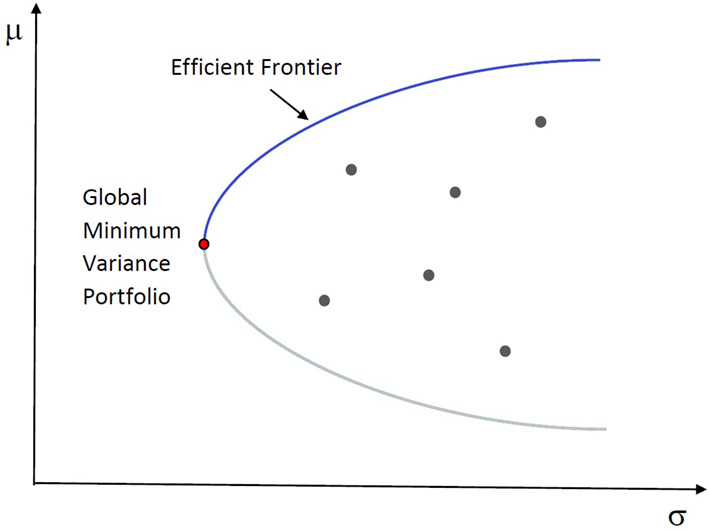
\includegraphics[scale=0.4]{GMV.jpg}
%  \caption{}
\end{figure}


\subsection{Tangency (Maximum Sharpe) Portfolio}
When a risk-free asset with rate $r_f$ is available, an important portfolio on the efficient frontier is the \emph{tangency portfolio}, which maximizes the Sharpe Ratio:
\[
\mbf w_{\mathrm{tan}}
~:=~
\underset{\mbf w}{\arg \max}
\;
\frac{\mbf w^\top \,\b \mu - r_f}{\sqrt{\mbf w^\top \,\mbf \Sigma \,\mbf w}}
\quad
\text{s.t.}
\quad
\left|
\begin{aligned}
& \mbf w^\top \,\mbf 1 = 1, \\
& w_i \,\ge\, 0~~\forall i ~~(\text{if short-selling is not allowed}).
\end{aligned}
\right.
\]
Geometrically, $\mbf w_{\mathrm{tan}}$ is the portfolio on the efficient frontier that yields the highest slope from $(0,r_f)$ to a point on the mean--variance graph. If $r_f$ is set to $0$, we maximize $\frac{\mbf w^\top \,\b \mu}{\sqrt{\mbf w^\top \,\mbf \Sigma \,\mbf w}}$.  

\begin{figure}[H]
  \centering
  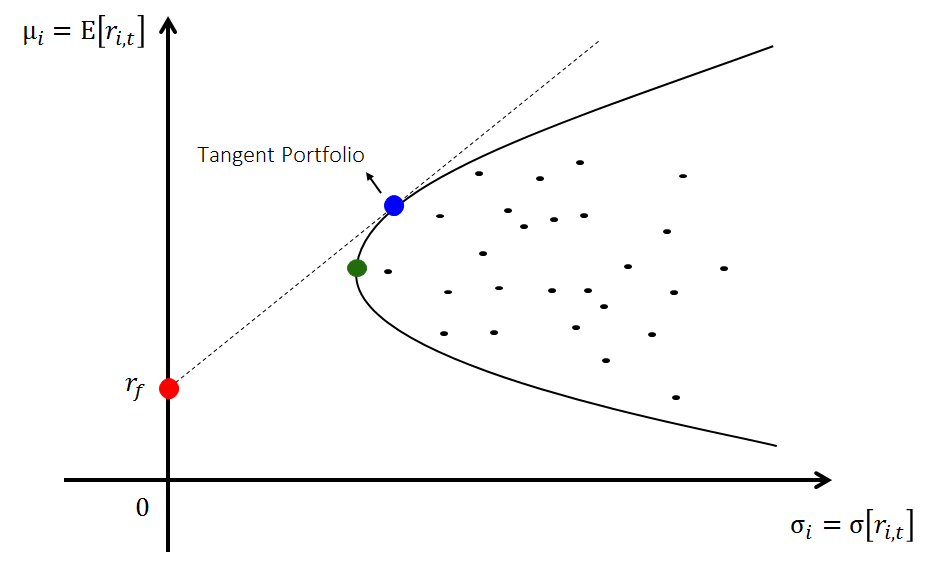
\includegraphics[scale=0.4]{tangency_portfolio.png}
%  \caption{}
\end{figure}


\subsection{Beyond Variance: Other Risk Measures}

\paragraph{General Form.} In place of minimizing $\mbf w^\top \,\mbf \Sigma \,\mbf w$, one can write an optimization problem of the form:
$$
\mbf w_{\mathrm{alt}}
~:=~
\underset{\mbf w}{\arg \min}
\;
\mathrm{Risk}\bigl(R^p\bigr)
\quad
\text{s.t.}
\quad
\left|
\begin{aligned}
%& \E \bigl[R^p\bigr] \;\ge\; \mu_{\min}, \\
& \mbf w^\top \,\mbf 1 = 1, \\
& \mbf w \,\ge\, \mbf 0.
\end{aligned}
\right.
$$
where $\mathrm{Risk}(\cdot)$ represents an alternative risk measure of the portfolio returns. 








\subsubsection{Value at Risk (VaR) and Expected Shortfall (ES)}
%While variance (or standard deviation) is the classical risk measure, many practitioners use alternatives that focus on downside risk.
Recall that \(R^p\) represents the \emph{return} of a portfolio. A \emph{negative} realization of \(R^p\) thus corresponds to a monetary loss, while a \emph{positive} realization corresponds to a gain. In many risk-management contexts, practitioners use \emph{Value at Risk} (VaR) and \emph{Expected Shortfall} (ES) (also called \emph{Conditional VaR}, CVaR) as \textbf{downside risk measures}. 

\paragraph{Value at Risk (VaR).}
For a given confidence level \(\alpha \in (0,1)\) (often \(\alpha=0.95\) or \(0.99\)), the \(\text{VaR}_\alpha(R^p)\) is interpreted as \emph{how large a loss} one might experience \emph{with small probability} \(1-\alpha\). Since a ``loss'' means \(R^p\) is negative, a common way to define VaR for a \emph{return} variable is
$$
\mathrm{VaR}_{\alpha}(R^p) 
~:=~
-\,q_{\,1-\alpha}(R^p),
$$
where \(q_{\,1-\alpha}(R^p)\) is the \((1-\alpha)\)\emph{-quantile} of \(R^p\). Concretely:
\[
\mathbb{P}(R^p \,\le\, q_{1-\alpha}(R^p)) \;=\; 1-\alpha.
\]
Because \(q_{1-\alpha}(R^p)\) is typically a negative number for high \(\alpha\), multiplying by \(-1\) makes \(\mathrm{VaR}_\alpha(R^p)\) a nonnegative \emph{magnitude of potential loss}. For instance, if \(\alpha = 0.95\) and we find \(\mathrm{VaR}_{0.95}(R^p) = 5\%\), that suggests a \emph{5\% loss} could occur in the worst 5\% scenarios (equivalently, with probability \(1-\alpha=0.05\)).

\paragraph{Expected Shortfall (ES) or Conditional VaR.}
Expected Shortfall (ES) at level \(\alpha\) refines VaR by considering \emph{the average loss} in those worst \((1-\alpha)\) scenarios where \(R^p\) is at or below its \((1-\alpha)\)-quantile. Formally:
\[
\mathrm{ES}_{\alpha}(R^p)
~:=~
-\,\frac{1}{1-\alpha}
\int_{0}^{\,1-\alpha}
q_{\,u}(R^p)
\;\mathrm{d}u,
\]
where \(q_{\,u}(R^p)\) is the \(u\)-quantile of \(R^p\). Equivalently, if \(\zeta = q_{\,1-\alpha}(R^p)\) is the VaR threshold (a negative return), then
\[
\mathrm{ES}_{\alpha}(R^p)
~=~
-\E\2{R^p \c R^p \leq \zeta },
\]
again producing a \emph{nonnegative} risk measure. In words, \(\mathrm{ES}_{\alpha}(R^p)\) looks at the average shortfall \(\bigl|R^p\bigr|\) (the \emph{magnitude of negative return}) on all occasions when \(R^p\) is at least as bad as the VaR threshold.

%\paragraph{Replacing Variance with VaR or ES in Optimization.}
%When we use these risk measures to build \emph{downside-focused} portfolios, we replace the classical variance objective or constraint with VaR or ES. For instance, in place of
%\[
%\min_{\mbf w} \;\mbf w^\top \mbf \Sigma \,\mbf w,
%\]
%we might solve:
%\[
%\min_{\mbf w}
%\;\mathrm{VaR}_{\alpha}\bigl(R^p\bigr)
%\quad\text{or}\quad
%\min_{\mbf w}
%\;\mathrm{ES}_{\alpha}\bigl(R^p\bigr),
%\]
%subject to a required minimum expected return, budget constraints, etc. In the case of ES (CVaR), this often leads to a \emph{convex} optimization problem (especially under scenario-based or parametric models), making it numerically tractable in many practical settings.

\begin{figure}[H]
  \centering
  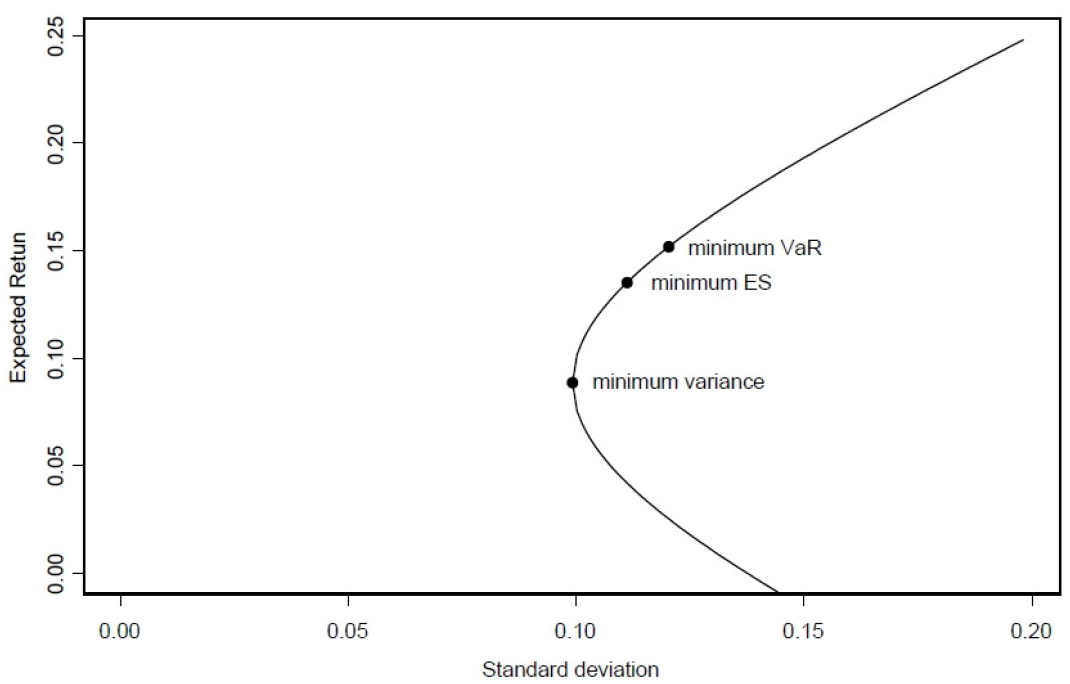
\includegraphics[scale=0.4]{CVAR_ES.png}
%  \caption{}
\end{figure}
